\begin{atiTask}[
  title = Vektoroperatoridentitäten I
  %call = Zusatzaufgabe,
]
%SoSe17 blatt 5 /4 ohne i) und ohne b)
%\begin{atiSubtasks}
Bestätigen Sie im Indexkalkül folgende Identitäten:
\begin{atiSubequations}
%\item{\divergence(\lambda \vec{a})=\vec{a}\grad{\lambda}+\lambda\divergence{a}
\item{\curl (\lambda \vec{a})=(\gradient \lambda)\times \vec{a}+\lambda \curl \vec{a}}
%
\item{\gradient(UV)=U\gradient V+V\gradient U}
%
\item{\divergence (\vec{a}\times\vec{b})=\vec{b}\curl \vec{a}-\vec{a}\curl \vec{b}}
%
\item{\gradient(\vec{a}\vec{b})=(\vec{b}\gradient)\vec{a}+(\vec{a}\gradient)\vec{b}+\vec{a}\times \curl \vec{b}+\vec{b}\times \curl \vec{a}}
%
\item{\curl (\vec{a}\times \vec{b})=(\vec{b}\gradient )\vec{a}-(\vec{a}\gradient)\vec{b}+\vec{a}\divergence \vec{b}-\vec{b}\divergence \vec{a}}
%
\item{(\vec{a}\gradient )\vec{a}=-\vec{a}\times \curl \vec{a}, \quad \text{wenn}\quad \vec{a}^2=\text{const}}
\item{\Delta (UV)=U\Delta V+V\Delta U+2\gradient U \cdot \gradient V}
\end{atiSubequations}
%\end{atiSubtasks}

\end{atiTask}

\begin{atiSolution}
	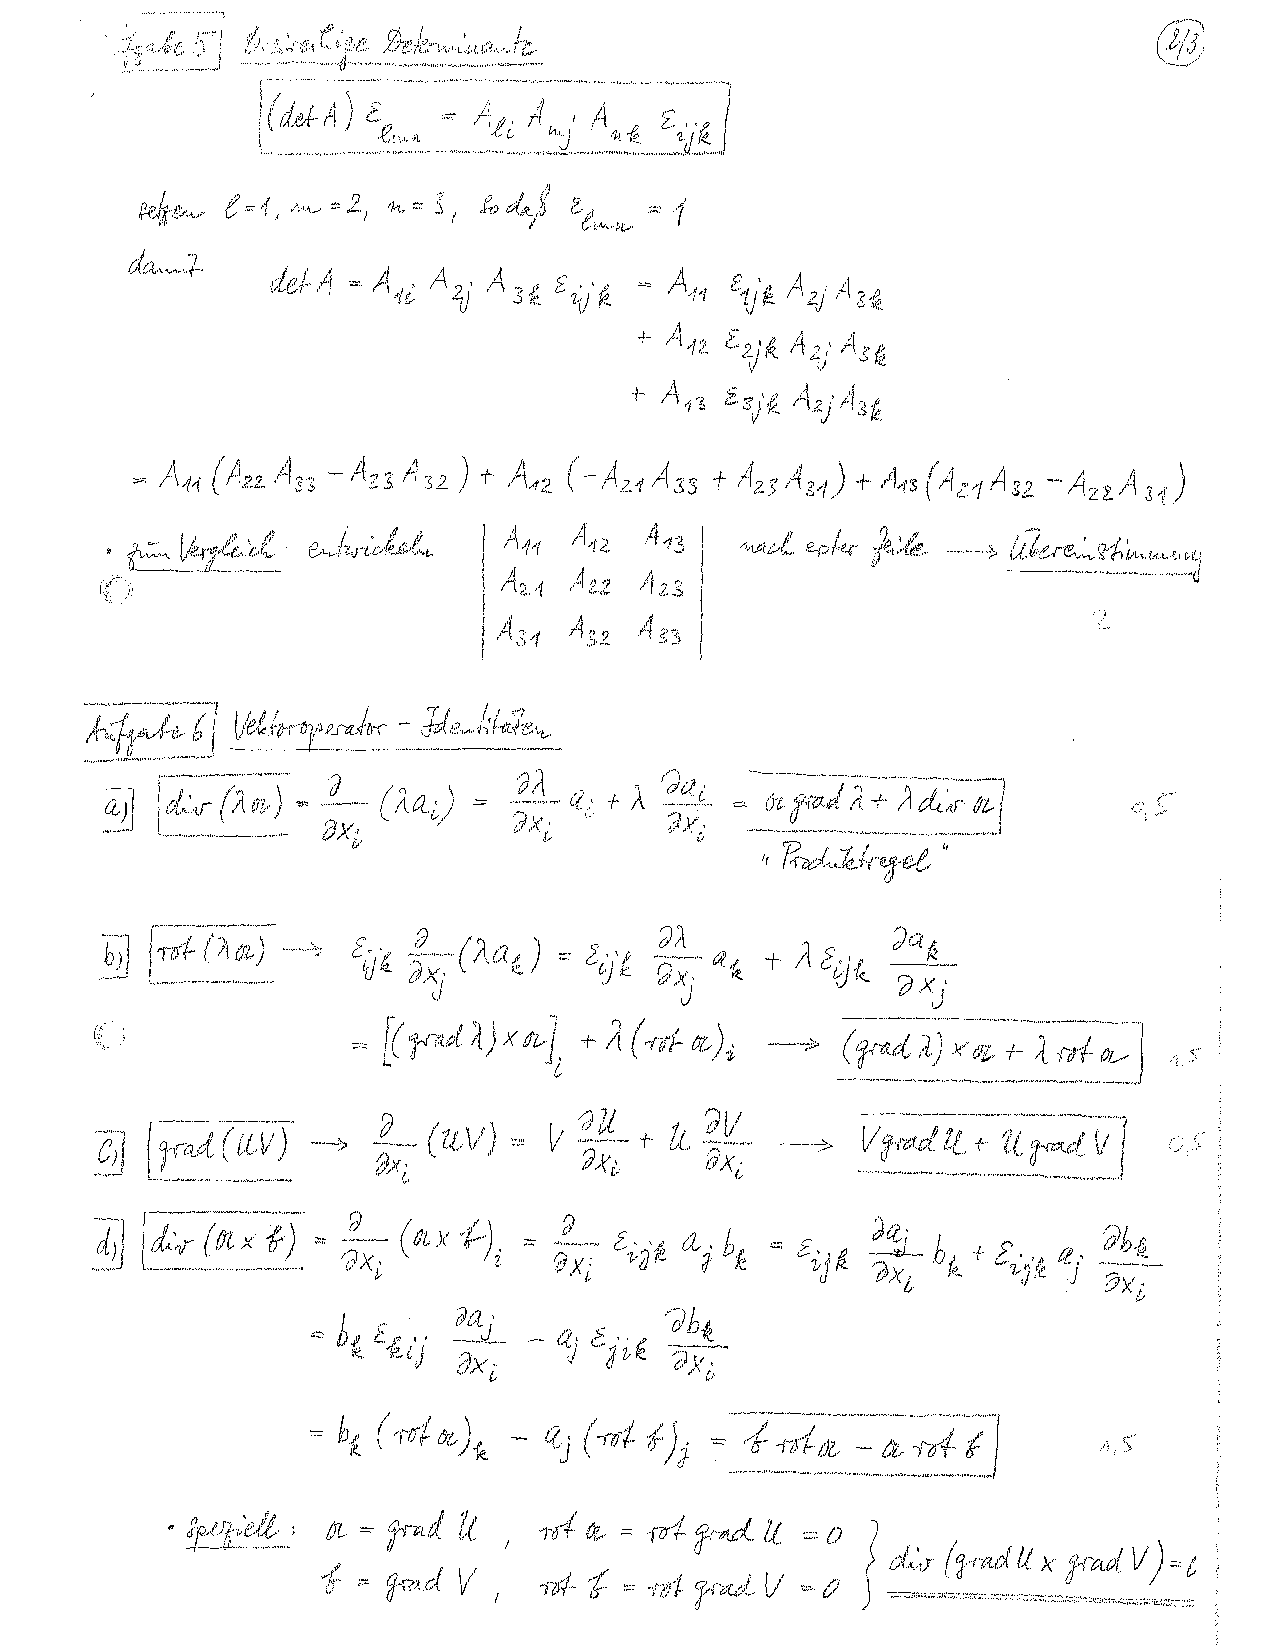
\includepdf[pages=-]{solution-index_i.pdf}
\end{atiSolution}